%% project.tex
%% 2015/12/05
%% by Eric Scott Freeman
%% This document uses bare_jrnl_compsoc.tex template provided by Michael Shell.

\documentclass[10pt,journal,compsoc]{IEEEtran}

\ifCLASSOPTIONcompsoc
	% The IEEE Computer Society needs nocompress option
	% requires cite.sty v4.0 or later (November 2003)
	\usepackage[nocompress]{cite}
\else
	% normal IEEE
	\usepackage{cite}
\fi

\newcommand\MYhyperrefoptions{bookmarks=true,bookmarksnumbered=true,
	pdfpagemode={UseOutlines},plainpages=false,pdfpagelabels=true,
	colorlinks=true,linkcolor={black},citecolor={black},urlcolor={black},
	pdftitle={Anti-plagiarism Project},
	pdfsubject={Anti-plagiarism},
	pdfauthor={Eric Scott Freeman},
	pdfkeywords={anti-plagiarism, plagiarism, fingerprinting, stylometry, Moss, JPlag, dupl, Autograder}}

\usepackage{amssymb}                % For the checkmarks in the table
\usepackage{booktabs}               % For the table
\usepackage{floatrow}               % To make the images fit
\usepackage{graphicx}               % To show images
\usepackage{listings}
\usepackage{url}                    % For adding URLs
\usepackage[utf8]{inputenc}         % For displaying accented characters

% correct bad hyphenation here
\hyphenation{}

\begin{document}

	\title{Anti-plagiarism Project}
	\author{Eric~Scott~Freeman}

	\IEEEtitleabstractindextext{
	\begin{abstract}
	This project integrates several anti-plagiarism tools into Autograder, software used by the University of Stavanger to automatically grade students' programming assignments. The three tools used were good at finding duplicate pieces of code, but it is still up to the instructor to determine whether or not it could be considered plagiarism.
	\end{abstract}
		
	\begin{IEEEkeywords}
	anti-plagiarism, plagiarism, fingerprinting, stylometry, Moss, JPlag, dupl, Autograder.
	\end{IEEEkeywords}}

	\maketitle
	\IEEEdisplaynontitleabstractindextext
	\IEEEpeerreviewmaketitle

	\IEEEraisesectionheading{\section{Introduction}\label{sec:introduction}}
	
	\IEEEPARstart{T}{he} University of Stavanger uses an application called Autograder, written by Heine Furubotten, to automatically grade students' programming assignments. Autograder works with GitHub. Whenever a student pushes their code to GitHub, Autograder will pull a copy of the code and run a series of tests on it. Autograder does not currently have support for plagiarism detection. The goal of this project is to integrate a few anti-plagiarism tools into Autograder, thereby helping professors save time.

	\section{Related Work}
	Unfortunately software plagiarism is a problem both in the classroom and in the workplace. A number of applications have been created to help detect this problem. While these tools can detect similarities in programs, the flagged files must still be manually examined to determine whether or not code was plagiarized.
		
	There are several different general techniques that are used to look for plagiarism. The tools analyzed in this project used either fingerprinting or stylometry.
		
		\subsection{Fingerprinting}
		Several tools use a technique called fingerprinting to detect plagiarism. In fingerprinting algorithms, hashes of $n$-grams, substrings that are $n$ characters, are saved and compared to help find plagiarism. Not all hashes are stored due to the large number that would be produced. 
		
			\subsubsection{Winnowing}
			Moss uses a technique called winnowing to select which hashes to save \cite{schleimer+wilkerson+aiken}. In the winnowing algorithm, a window, selection of contiguous hashes, is used to help select which hashes to save. The smallest hash from a window is saved, and then the window moves one hash over. The smallest hash from the next window is often the smallest hash from the previous window. If so it is not saved again. Figure \ref{fig:winnowing1} shows an example of how winnowing works. The orange box represents the shifting window. The green box shows whenever a new hash is saved.
		
			\begin{figure}[h!]
				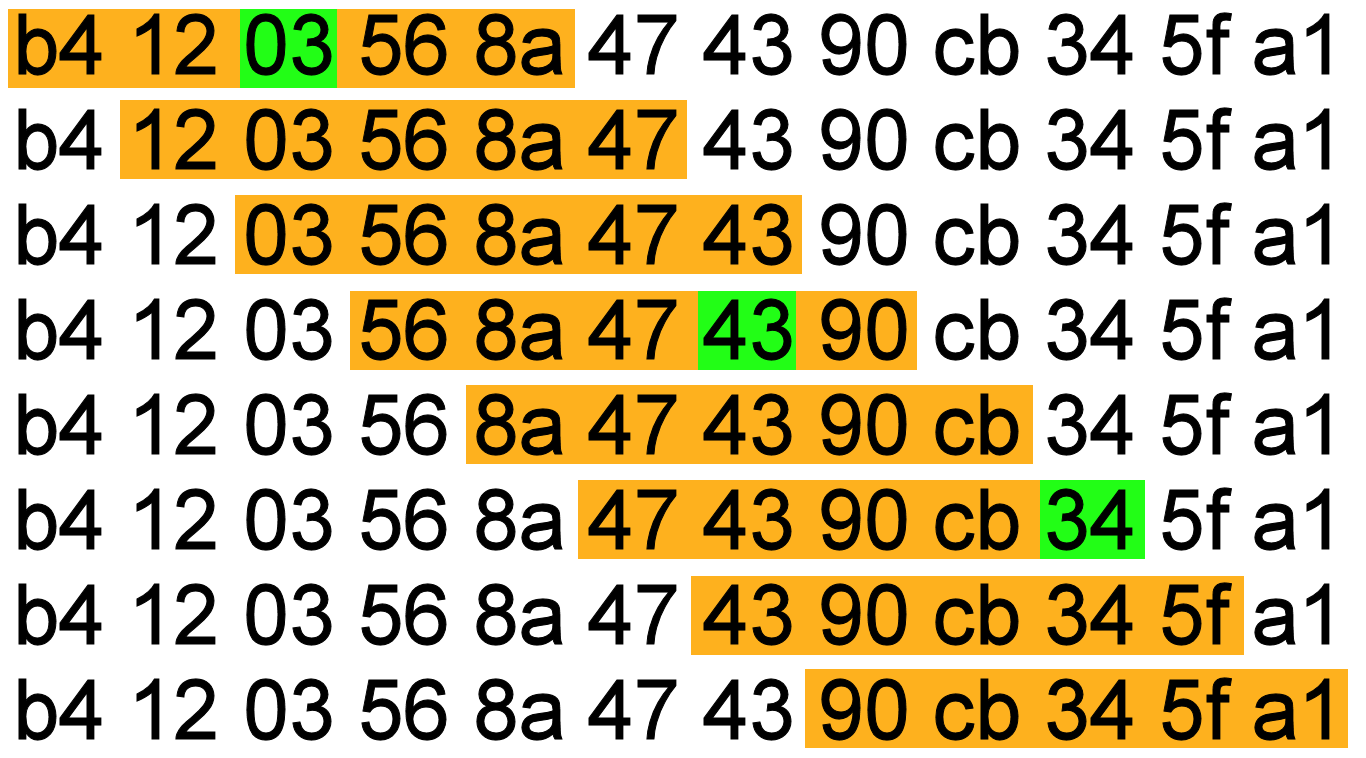
\includegraphics[width=0.8\textwidth]{Winnowing.png}
				\caption{Winnowing.}
				\label{fig:winnowing1}
			\end{figure}
		
			\subsubsection{Running-Karp-Rabin Greedy-String-Tiling}
			JPlag uses Running-Karp-Rabin Greedy-String-Tiling (RKS-GST) to compare hashes of code in plagiarism detection \cite{prechelt+malpohl+philippsen}. RKS-GST was originally used in YAP3, another plagiarism detection tool. In RKS-GST, the Greedy String half of the algorithm forms pairs of substrings, each from a different string. Then the Karp-Rabin half of the algorithm hashes each substring in the pair \cite{wise}. This is done to help detect code reordering.
		
		\subsection{Stylometry}
		Another approach is to use code stylometry, which analyzes the style of writing or coding.
		
			\subsubsection{Abstract Syntax Trees}
			Caliskan-Islam, et al. use abstract syntax trees (ASTs) to compare the styles of authors \cite{caliskan-islam+harang+liu}. Things that are easily changed in code, such as variable names, become leaves in the AST, while the structure of the tree is harder to change \cite{caliskan-islam+harang+liu}. Figure \ref{fig:ast} shows an abstract syntax tree of the code in Figure \ref{fig:astcode}. Note how the leaves, or circular nodes, in Figure \ref{fig:ast} are variable names, constants, and a function name.
		
			Michal Bohuslávek's dupl application uses ASTs to find similarities in code \cite{bohuslave}. It looks for any copies of code, not just plagiarism. So if a piece of code is duplicated even in the same file, it will test positive.
		
			\begin{figure}
				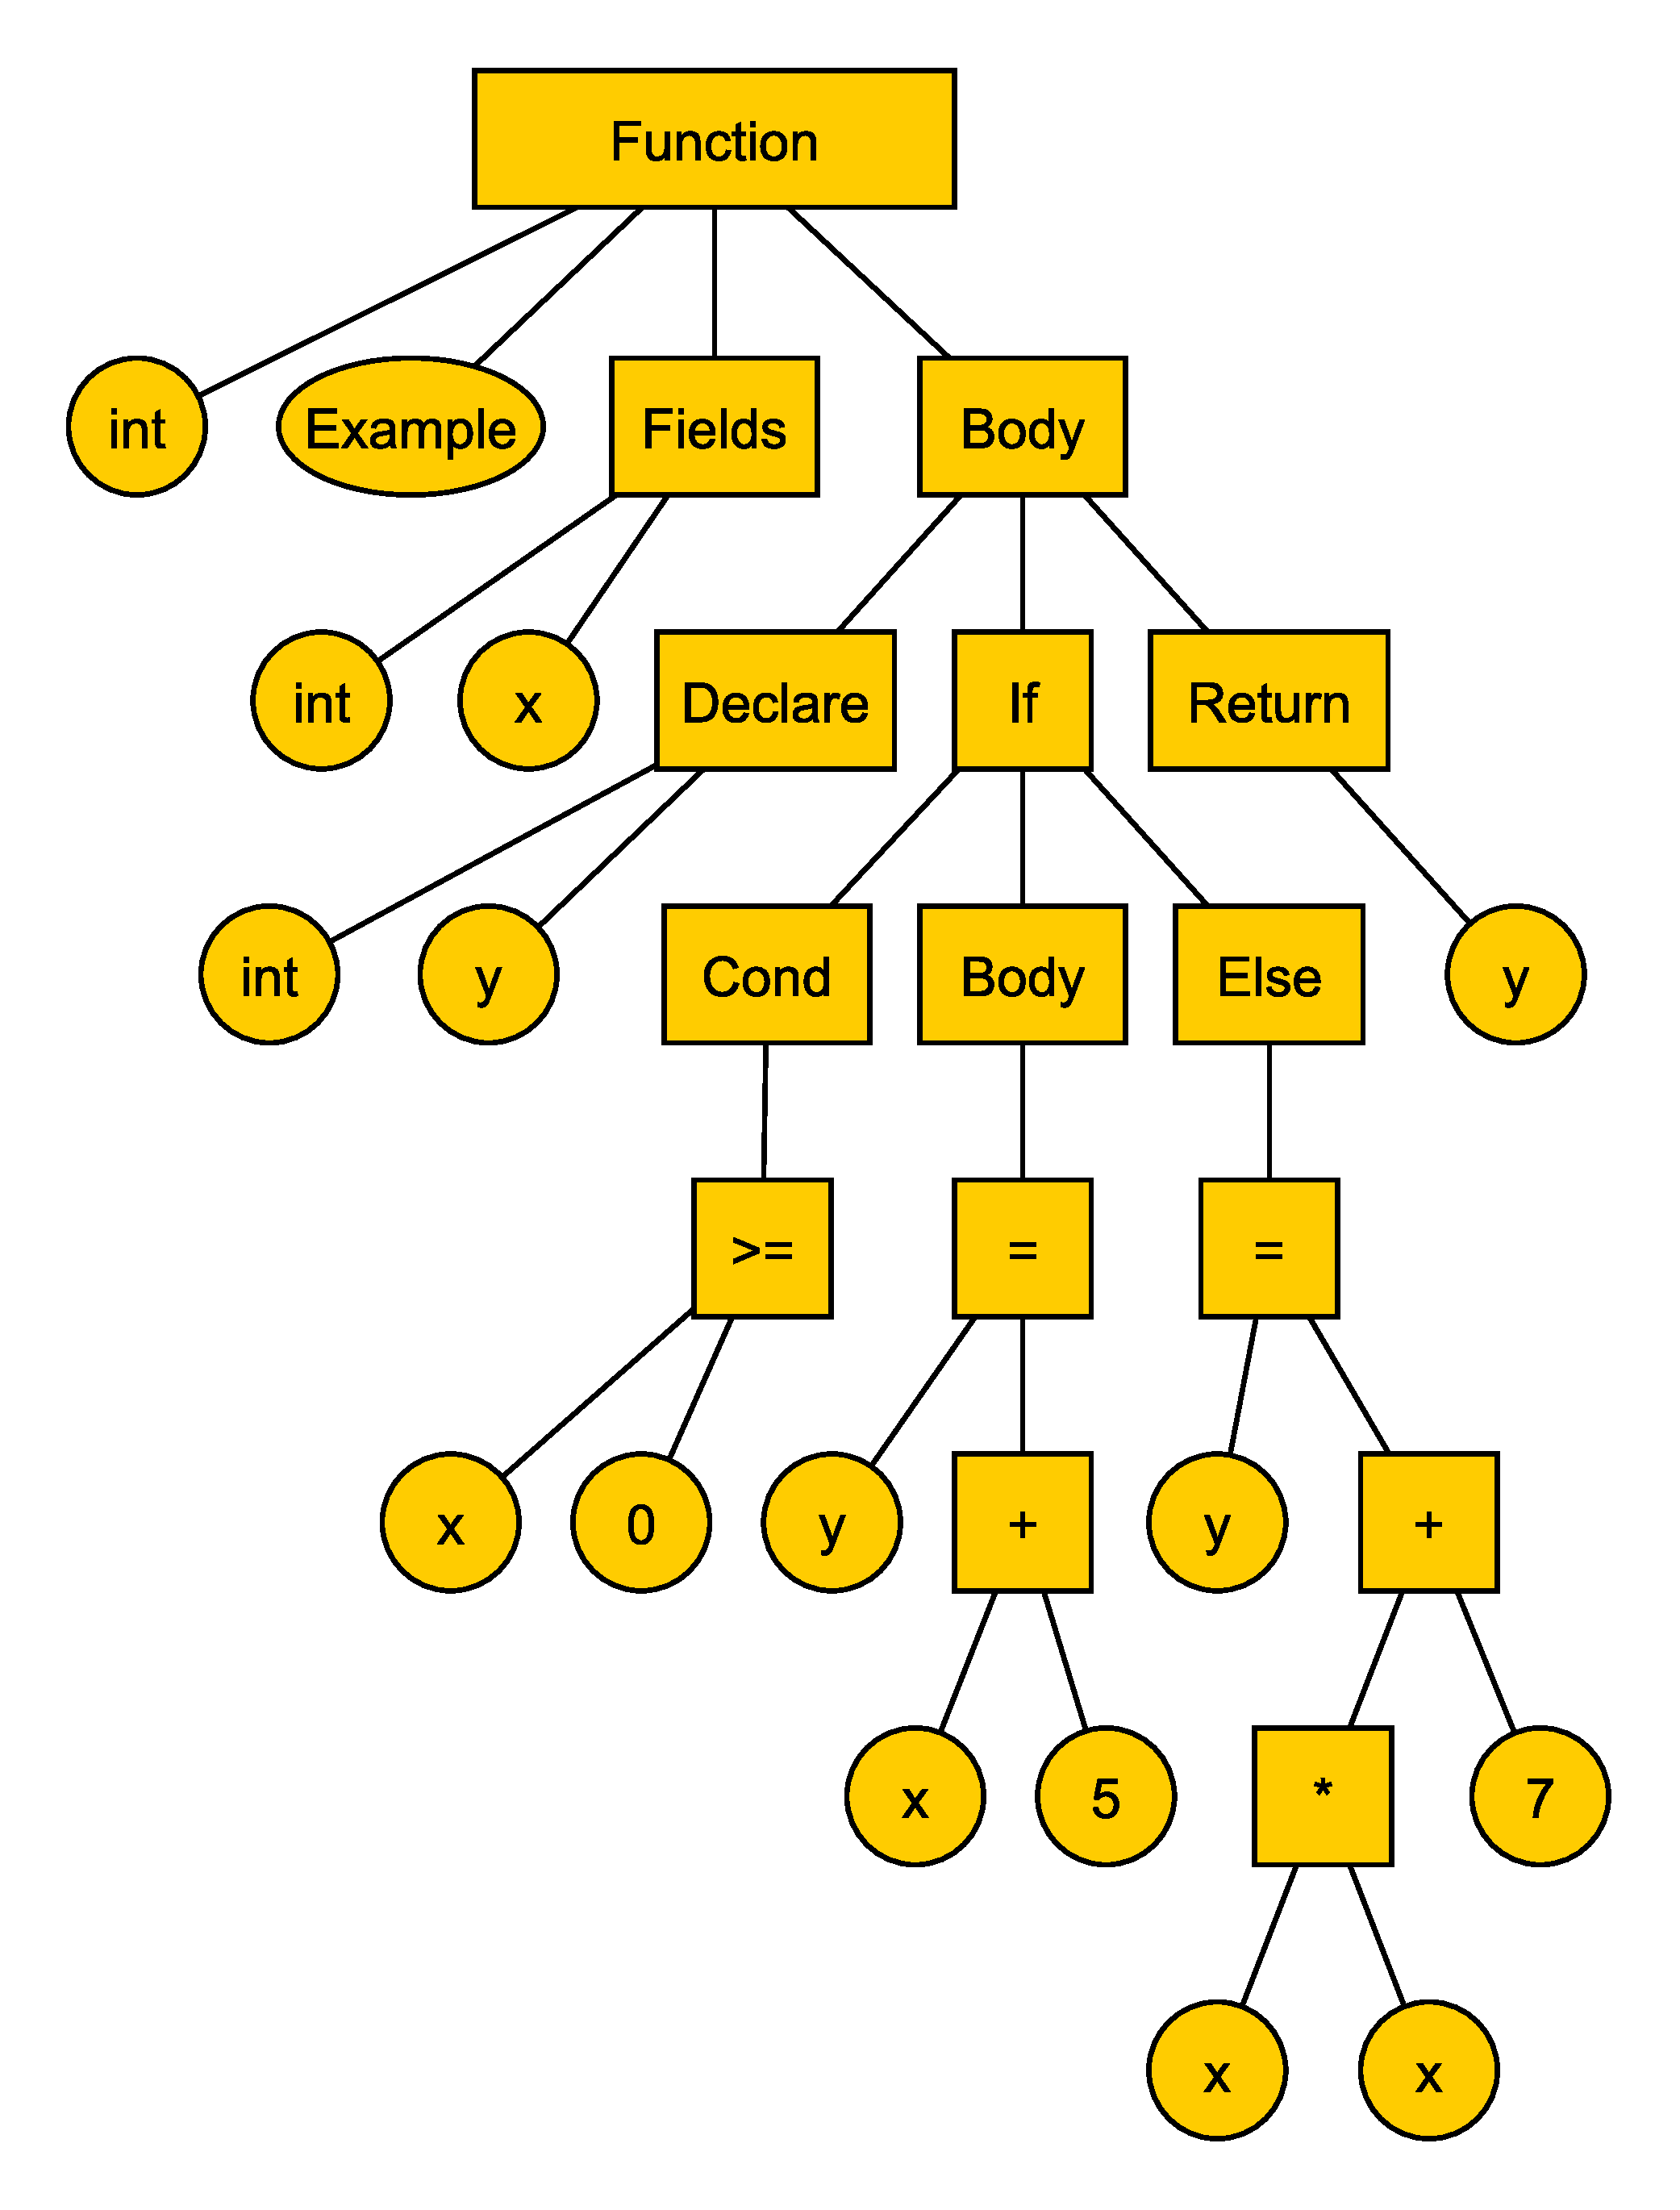
\includegraphics[width=0.8\textwidth]{AST.pdf}
				\caption{Abstract syntax tree.}
				\label{fig:ast}
			\end{figure}
			\begin{figure}
				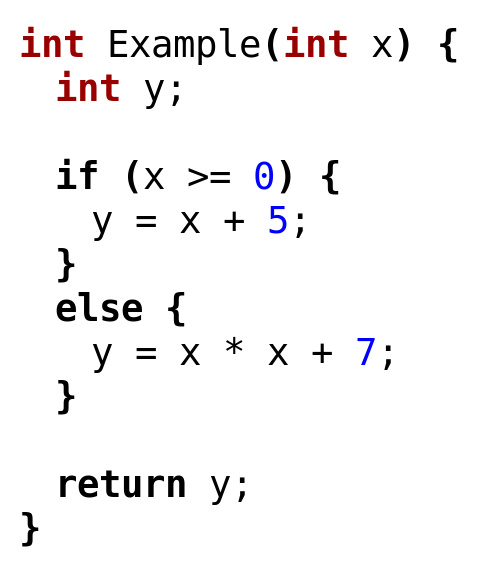
\includegraphics[width=0.5\textwidth]{ASTcode.png}
				\caption{Example code.}
				\label{fig:astcode}
			\end{figure}
		
		\subsection{Supported Languages}
		Fingerprinting and string comparison techniques can be used to analyze source code written in languages other than their officially supported languages. Moss can analyze Go code, even though it is not technically supported. Since ASTs need to parse the code, applications which use them are stricter on which languages they can analyze. For example dupl only supports code written in Go. Table \ref{tab:languageSupport} shows the languages officially supported by several anti-plagiarism tools.
		
		\begin{table}[h!]
			\begin{center}
				\caption{Officially supported languages by various tools}
				\label{tab:languageSupport}
				\begin{tabular}{ccccccccccccccc}
					\toprule
					Tool & Java & Go & C & C\verb!++! & C\verb!#! & Python & others\\
					\midrule
					Moss & \checkmark & & \checkmark & \checkmark & \checkmark & \checkmark & \checkmark \\
					JPlag & \checkmark & & \checkmark & \checkmark & \checkmark & & \checkmark\\
					Plaggie & \checkmark & & & & & & \\
					SIM & \checkmark & & \checkmark & & & & \checkmark\\
					dupl & & \checkmark & & & & & \\
					\bottomrule
				\end{tabular}
			\end{center}
		\end{table}
	\section{Design}
		\subsection{Selection of tools}
		Moss was the first choice in anti-plagiarism tools, because it supports a large number of languages and is a mature piece of software. Two other tools were added later: JPlag and dupl. Like Moss, JPlag supports many languages. While dupl is less than a year old, it uses ASTs. These three tools allow the project to use three different techniques for finding plagiarism: winnowing, RKS-GST, and ASTs.

		\subsection{Process}
		Since Autograder was written in Go, this project was also written in Go. Later it was decided to make this project a standalone application that Autograder will call, since another university has expressed interest in using it. The program calls each of the anti-plagiarism tools and stores the results. A separate Go package was written for each anti-plagiarism tool. The packages implement a common interface which creates the commands to send to the tools and formats the results. The interface will allow other anti-plagiarism tools to be easily added later.
		
		The anti-plagiarism application typically runs as a service and accepts gRPC, a remote procedure call framework, requests. A request consists of the GitHub organization, the GitHub authorization token, an array of student repository names, and an array of lab assignment names and programming languages. Requests can also be sent from the command line.
		
		The \verb|golint| application was run against the code for suggestions on making the code follow Go coding conventions. The \verb|go fmt| command was run to clean up the whitespace in the code.
	
			\subsubsection{Calling the anti-plagiarism tools}
			Before calling the anti-plagiarism tools, first the students' code is pulled from GitHub to the Autograder server. The directory structure consists of a base directory containing subdirectories for each class. Each class is a GitHub organization. Inside each class, there are directories for each student, which have directories for each assignment. See figure \ref{fig:directories}. This is similar to how Autograder stores the files in GitHub, so pulling the code for the anti-plagiarism project is simplified.
	
			\begin{figure}[h!]
				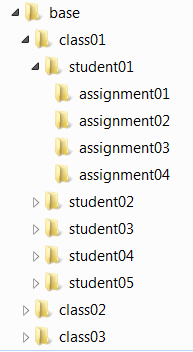
\includegraphics[width=0.4\textwidth]{Directories.png}
				\caption{Directory structure.}
				\label{fig:directories}
			\end{figure}
			
			\begin{figure}[h!]
				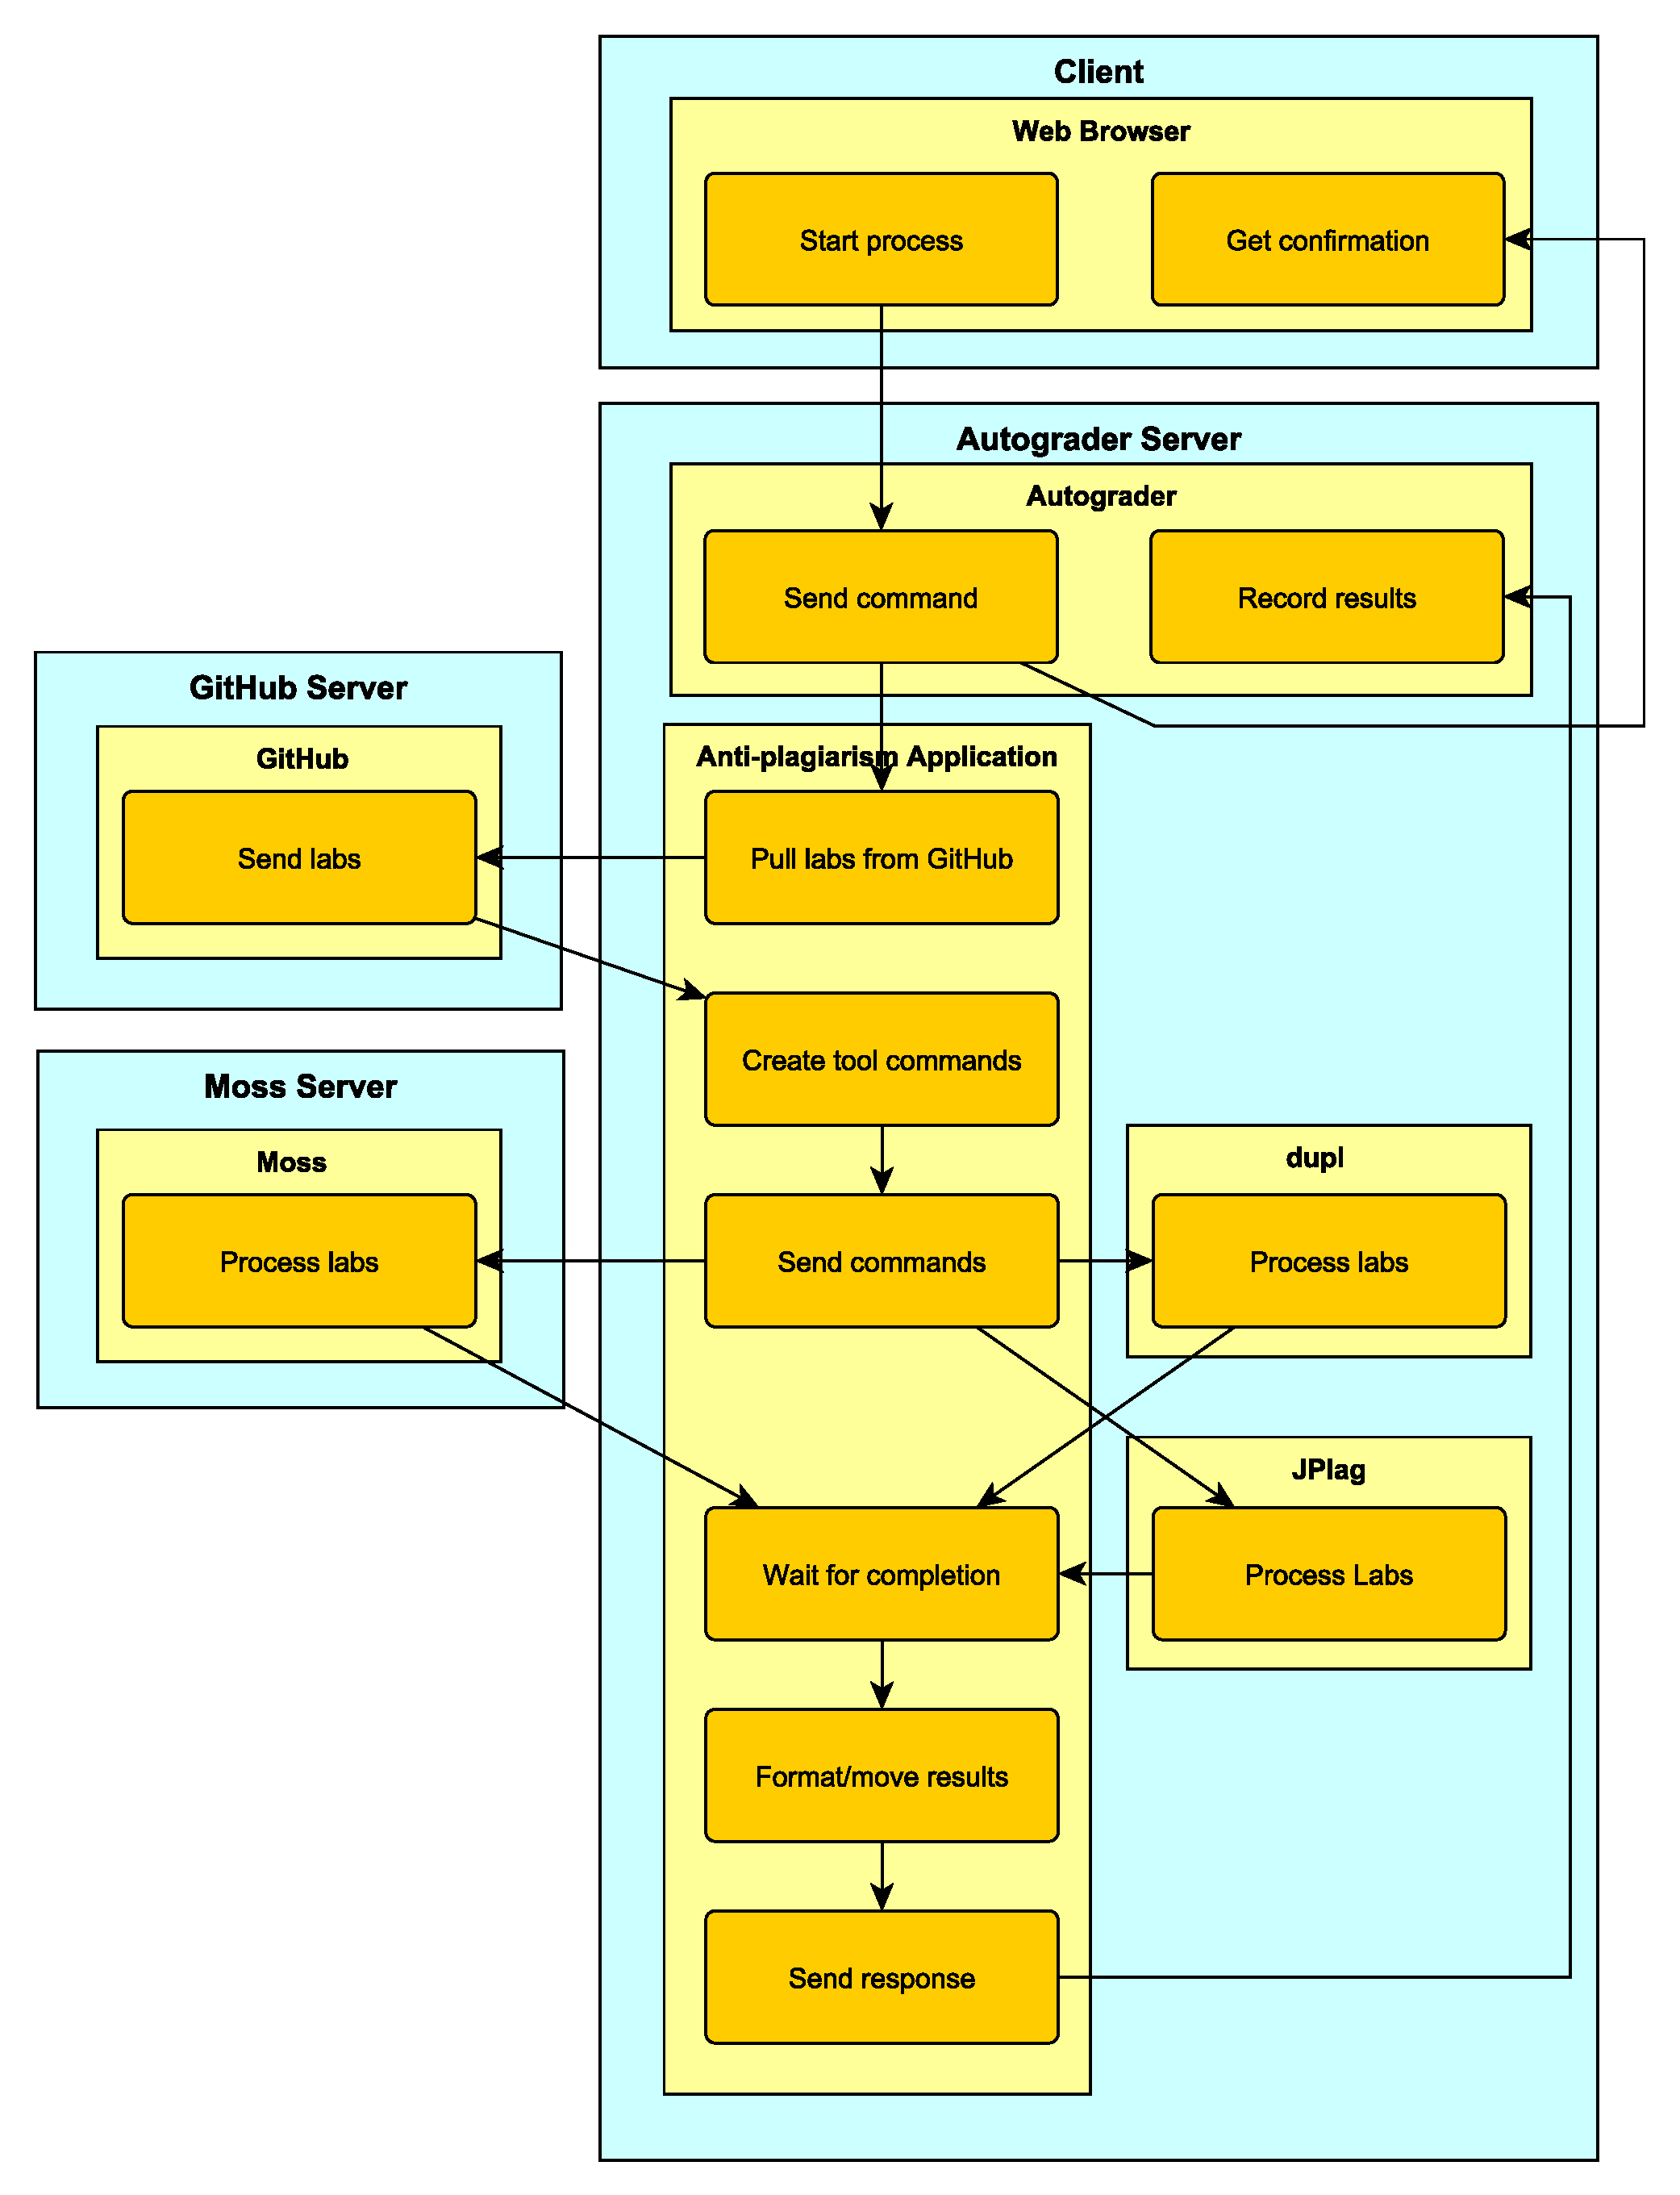
\includegraphics[width=1.0\textwidth]{process2.pdf}
				\caption{Process}
				\label{fig:process}
			\end{figure}
	
			Next the commands are created for each anti-plagiarism tools based on the location of the code, the language in which the code was written, the threshold of the tool, and various other parameters. The commands are then sent to their respective tools. Each student's work for an assignment is compared against the other students' work for that particular assignment in that class instead of all the assignments for that class or all the assignments for all classes. This keeps the number of files being compared from growing too large.
			
			The anti-plagiarism application waits for the results to come back from each of the tools. When they have all finished, the program will collect and store the resulting HTML files in the location specified. It also examines the HTML files for the highest incidents of plagiarism for each student. The highest values are written to a JSON file. Finally the program sends a gRPC response back to the calling application indicating if it was successful or not.
			
		\subsection{Integrating with Autograder}
		A few new fields needed to be added to the Autograder's Bolt database. Bolt stores entries as a key/value pair. Each lab assignment entry in each class needed to store the language the assignment is written in. Also each lab assignment entry for each student/group needed to store the results from each of the anti-plagiarism tools.
		
		The user interface was also updated to allow teachers to assign a programming language to each lab (figure \ref{fig:selectLang}), to allow teachers to initiate the anti-plagiarism process (figure \ref{fig:startTest}), and to show the results of the process. When the Autograder web service receives a request to start the anti-plagiarism process, it creates the gRPC command. If it was successful it sends the request and informs the user that the request was sent. Since it can take at least several minutes to process the data, it is best to inform the user immediately that things might take a while. Otherwise they could think that it is not working. Then Autograder starts a Go routine (separate thread) to call the anti-plagiarism software and process the results.
		
		\begin{figure}[h!]
			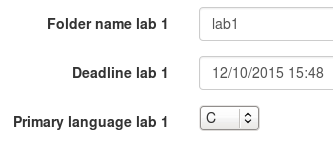
\includegraphics[width=0.6\textwidth]{SelectingLanguage.png}
			\caption{Selecting language.}
			\label{fig:selectLang}
		\end{figure}
				
		\begin{figure}[h!]
			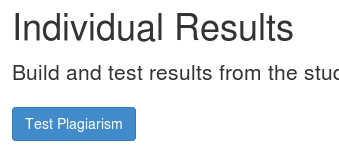
\includegraphics[width=0.6\textwidth]{StartTest.png}
			\caption{Start anti-plagiarism test.}
			\label{fig:startTest}
		\end{figure}
		
		The results are stored in the database and also displayed to the teachers through the teacher panel in Autograder. The teacher panel shows a table of all the students in the class and their assignments. If any of the anti-plagiarism tools find evidence of plagiarism, the corresponding cell in the table will be colored a shade of red. The more tools finding plagiarism, the deeper the color. From the teacher panel, teachers go to a results page to look at more details about each lab. This page shows the results of each anti-plagiarism tool and buttons to show the plagiarized code. See figure \ref{fig:labresults}.
		
		\begin{figure}[h!]
			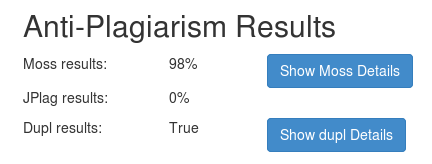
\includegraphics[width=0.7\textwidth]{LabResults.png}
			\caption{Results for one lab.}
			\label{fig:labresults}
		\end{figure}
		
		While adding the new functionality to Autograder, care was taken not to break any existing functionality. Unit tests were rerun to check that nothing was broken.
		
	\section{Results}
	
		\subsection{Choosing threshold values}
		Choosing threshold values took some consideration plus trial and error. Since the threshold value for Moss is the number of files duplicate code can appear in and still be considered plagiarism, it was straightforward to find a value for Moss. The test class consisted of seventeen students and six groups. Therefore the Moss threshold would need to be less than six, because all of the groups would have code provided by the instructor. So the value chosen was five.
		
		For JPlag and dupl, the threshold represents the number of tokens to compare. It was not known how much data a token represents in JPlag, but luckily the output included the number of tokens in each match. In figure \ref{fig:jplag20} it is shown that 20 tokens can match short functions that only print a value. In figure \ref{fig:jplag30} it is shown that 30 tokens can match a long list of variable assignments. Figure \ref{fig:jplag40} shows that 40 tokens will match pieces of code that are more substantial. Therefore a JPlag threshold of 35 was chosen to get better matches.
		
		\begin{figure}[h!]
			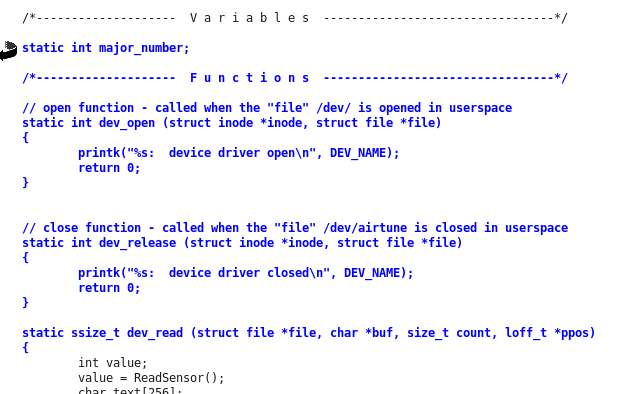
\includegraphics[width=0.6\textwidth]{jplag20.png}
			\caption{JPlag match with 20 tokens.}
			\label{fig:jplag20}
		\end{figure}
		
		\begin{figure}[h!]
			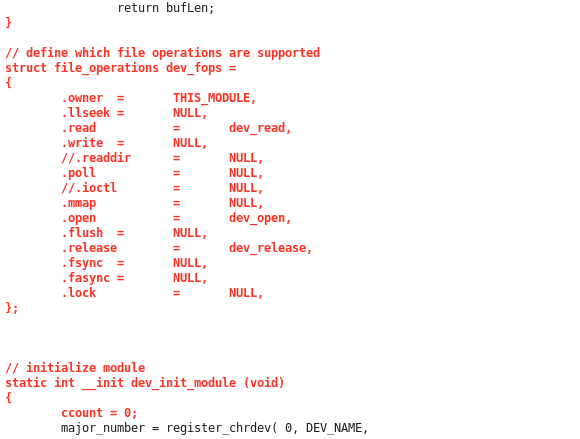
\includegraphics[width=0.4\textwidth]{jplag30.png}
			\caption{JPlag match with 30 tokens.}
			\label{fig:jplag30}
		\end{figure}
		
		\begin{figure}[h!]
			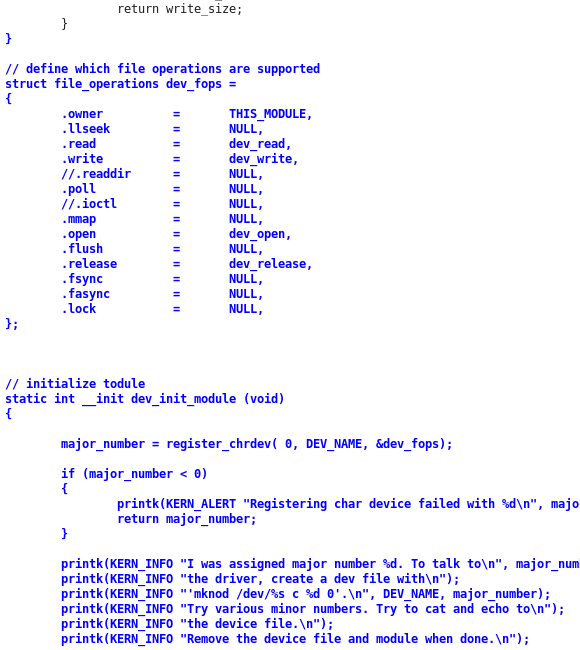
\includegraphics[width=0.8\textwidth]{jplag40.png}
			\caption{JPlag match with 40 tokens.}
			\label{fig:jplag40}
		\end{figure}
		
		Unfortunately dupl does not provide the number of tokens in a match. So the threshold value needed to be adjusted several times before some of the less detailed results were removed. Figure \ref{fig:dupl50} and figure \ref{fig:dupl75} show examples of matches when the threshold was set to 50 and 75 (up from the default value of 15). 75 was chosen for the final dupl threshold.
		
		\begin{figure}[h!]
			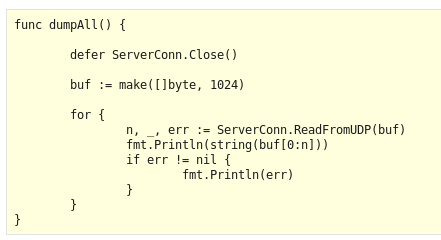
\includegraphics[width=0.5\textwidth]{dupl50.png}
			\caption{dupl match when threshold was 50 tokens.}
			\label{fig:dupl50}
		\end{figure}
		
		\begin{figure}[h!]
			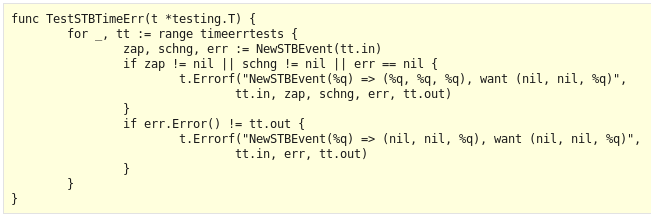
\includegraphics[width=1.0\textwidth]{dupl75.png}
			\caption{dupl match when threshold was 75 tokens.}
			\label{fig:dupl75}
		\end{figure}
		
		\subsection{Results in Autograder}
		
		Figures \ref{fig:indlabresults} and \ref{fig:grouplabresults} show the individual lab results and group lab results respectively for the test class. In labs one, five, and six, the students programmed in C. They programmed in Go for the remaining labs. All of the test code for the labs was written in Go.  Light pink indicates that one tool found duplicate pieces of code, and darker pink indicates two tools found duplicates. Three tools finding results will not occur because there is no overlap in the languages that JPlag and dupl can test.
		
		\begin{figure}[h!]
			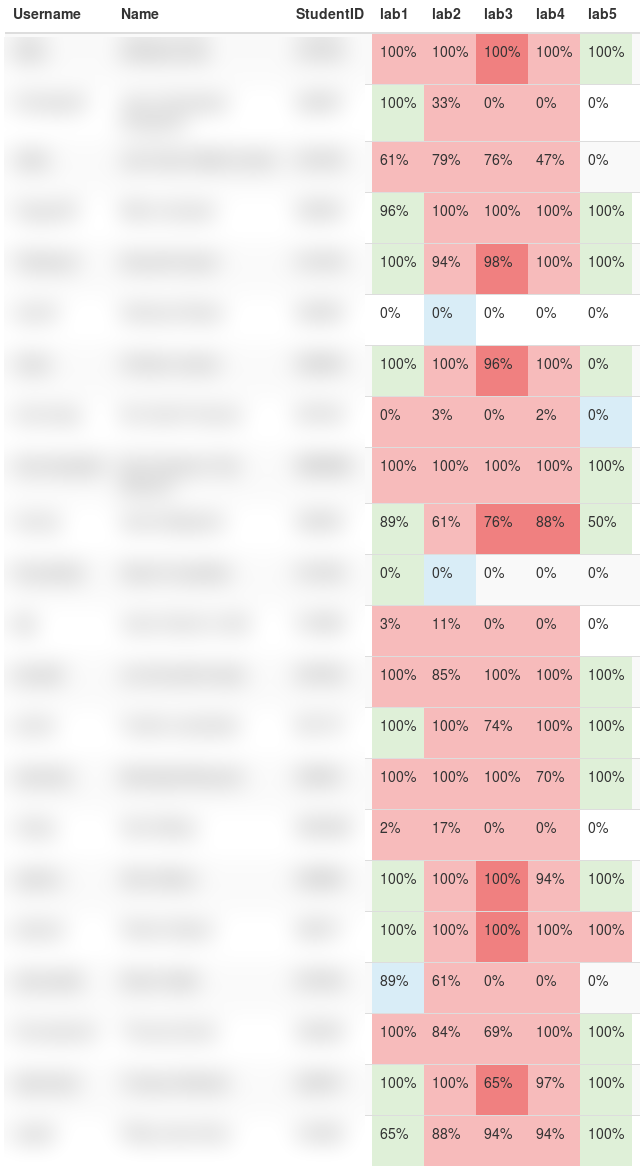
\includegraphics[width=0.5\textwidth]{indlabresults.png}
			\caption{Individual lab results. Instructors and TAs have accounts too.}
			\label{fig:indlabresults}
		\end{figure}
		
		\begin{figure}[h!]
			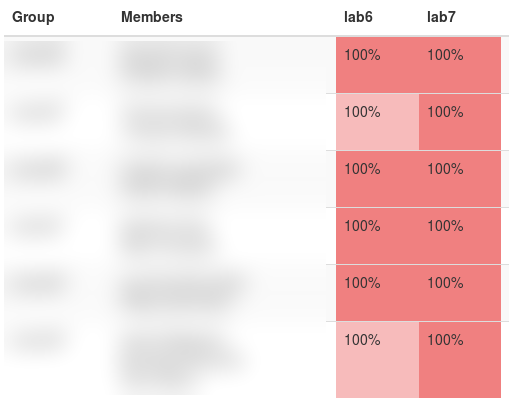
\includegraphics[width=0.3\textwidth]{grouplabresults.png}
			\caption{Group lab results.}
			\label{fig:grouplabresults}
		\end{figure}
	
	\section{Analysis}
	At first glance, it appeared as if all the students that submitted work plagiarized code, but that would be a very unlikely scenario. Most of the duplicates appear to come from code provided to the students. In labs one and five, little or no code was provided to the students. Therefore there were much fewer detections in these two assignments.
	
	Getting three separate tools to behave similarly using a common interface was a bit difficult. Moss was the original anti-plagiarism tool included in the project before it was decided to add other tools. Moss's threshold says to ignore code that is similar in a certain number of files. So if the threshold is ten and a piece of code appears at least ten times, it is not considered plagiarism. This is very helpful when an instructor gives students a partially completed file or a framework to follow. Since the threshold does not specify the length of code to consider for plagiarism, sometimes relatively short sections of code show up in the results. Unfortunately if a student's lab directory has subdirectories, Moss will say that similar code in different subdirectories is plagiarism.
	
	JPlag can produce false positives in two ways in this project. First, JPlag remembers the results from previous executions. So if a student uses a piece of code in one lab and then reuses the same piece of code in another lab, JPlag can detect this as plagiarism. The second way is JPlag is not ignoring code provided by the instructor. While it is possible to tell JPlag to ignore certain files, this would break the common interface shared among the tools. Also it would require the instructors to format the assignments in such a ways that all of the instructor provided code is separate from all of the student code.
	
	Dupl was not designed to detect plagiarism, only duplicate pieces of code. So it will detect all the instructor provided code as plagiarism. It can even detect two pieces of code in the same file. For example the two functions in figure \ref{fig:duplSameFile} are from the same file and are shown to be duplicates.
	
	\begin{figure}[h!]
		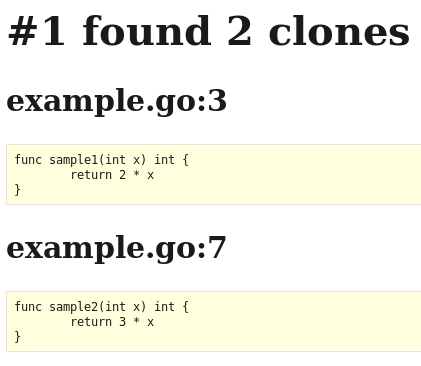
\includegraphics[width=0.7\textwidth]{duplSameFile2.png}
		\caption{Sample dupl results from same file.}
		\label{fig:duplSameFile}
	\end{figure}
	
	Since dupl is only looking for duplicate code and not plagiarism, it does not provide a number indicating the percentage of code it thinks is plagiarized. It also places all the results in a single HTML file rather than splitting them up into separate files.
	
	Adjustments were made to the thresholds in attempt to clean up the results shown in figures \ref{fig:indlabresults} and \ref{fig:grouplabresults}. Labs one and five improved some, but there was too much provided code in the other labs for cleaner results.
	
	\section{Future work}
	Currently the anti-plagiarism application is only intended to be called locally, so there is no encryption enabled in the gRPC calls. If it is to be called remotely, then transport security needs to be added in the anti-plagiarism application and in Autograder. If the application was called remotely, the result files would need to be sent to the other machine. There are also some hard-coded values in Autograder that should be environment variables or in a configuration file, such as the address and port of the anti-plagiarism application.
	
	Additional anti-plagiarism tools could be added later, but focusing on the use of one tool could be a better option. When using a common interface to access the different tools, some of the fine tuning is lost.
	
	Autograder does not do anything with the percentages other than display them. It could have its own threshold and only display results above a certain percentage.
	
	\section{Conclusion}
	Due to the high number of false positives found during testing, it is probably better to consider the results from this application as supplemental to any suspicions an instructor may have already. It would be tedious to examine all of the results. The tools used are very good at finding similar pieces of code, but there are legitimate reasons for having duplicate code, such as code distributed by the instructor or students reusing their own code. Use of this application is useful if an instructor suspects plagiarism and uses this to verify their suspicions.
	
	Results could be improved in future classes if all instructor provided code resided in separate repositories. This would greatly reduce the number of false positives. Then the work in the students' repositories would hopefully be their own work and not code copied from someone else.
	
	% use section* for acknowledgment
	\ifCLASSOPTIONcompsoc
		% The Computer Society usually uses the plural form
		\section*{Acknowledgments}
	\else
		% regular IEEE prefers the singular form
		\section*{Acknowledgment}
	\fi
	
	The author would like to thank Hein Meling for his advice and guidance during this project.
	
	\bibliography{sources}
	\bibliographystyle{ieeetr}

\begin{IEEEbiographynophoto}{Eric Scott Freeman}
is currently a master's student at the University of Stavanger. He received his Bachelor of Science degree in Computer Science from Midwestern State University in 2004. He has also worked as a software developer for several companies including RadioShack, Cisco Systems, and TelStrat.
\end{IEEEbiographynophoto}

\end{document}


